\chapter{Rover Controller Application}

\section{Overview} 
In order to provide an accessible, user-friendly interface to control the rover remotely, a web application has been developed. This application implements a back-end built with Express.js and a front-end with ReactJS.

\section{Front-end}
The front-end is the application's interface. In it, the user can control the rover and access information from it. It's main pages are the dashboard and the gallery.
\subsection{Dashboard}
In the dashboard, the user can interact with the rover and receive data from its sensors, using an MQTT client to control all data flows.
As soon as the dashboard is rendered, an MQTT client will be initiated and connected to the broker, then it will subscribe to all topics mentioned previously that the rover uses to send data.

The following image \ref{fig:web_dash} shows the implemented dashboard.
\begin{figure}[h]
    \centering
    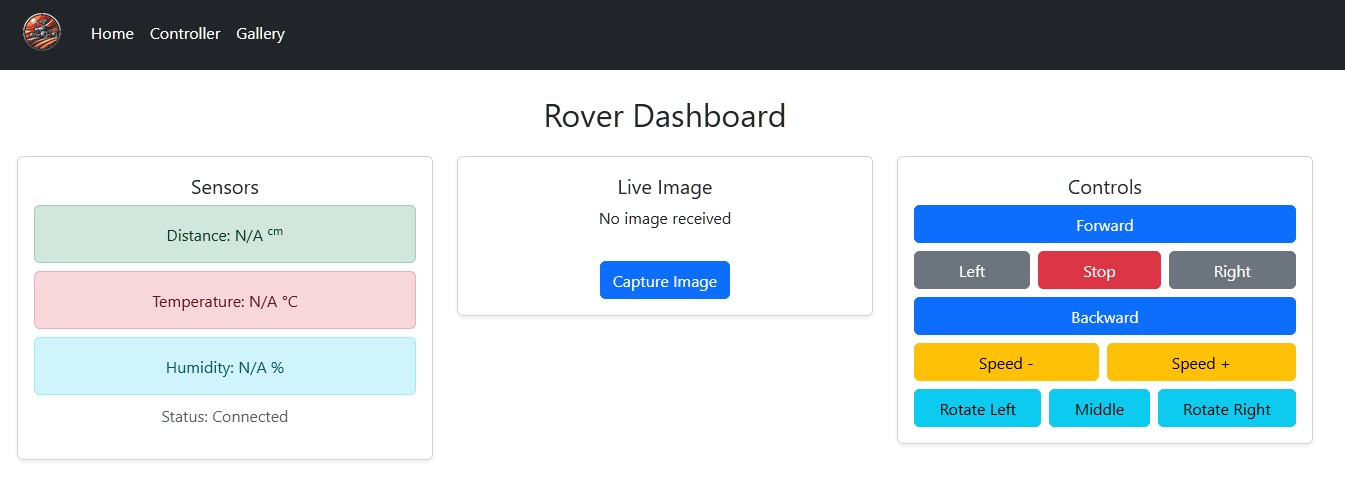
\includegraphics[width=1\linewidth]{Hauptkapitel/Pictures/App_dashboard.jpg}
    \caption{Rover's dashboard}
    \label{fig:web_dash}
\end{figure}
\paragraph{}The leftmost component shows the information gathered by the sensors, which gets updated as soon as new information gets sent and received. The middle component contains a button that publishes a command on \lstinline|iotrover/move| that makes the rover take and publish a photo through the topic \lstinline|photos|. 

%The photo will be retrieved as binary data and encoded to Base64 to show it on screen. At the same time, the image is sent to the back-end for it to be saved to the database.

The rightmost component contains a controller composed of multiple buttons. Each of these buttons will publish a command on the topic \lstinline|iotrover/move|, to which the rover is subscribed.

\subsection{Gallery}
This 